%----------------------------------------------------------------------------------------
% Chapter 1: Introduction
%----------------------------------------------------------------------------------------

\chapter{Introduction}
\label{ch:introduction}

%----------------------------------------------------------------------------------------

\section{Introduction}
\label{sec:introduction}

Modern recommendation systems are widely used in e-commerce platforms, video-streaming services, music applications, online marketplaces, and social-media platforms. These systems process large volumes of user--item interaction data generated through ratings, purchases, clicks, views, and other forms of explicit or implicit feedback. As the number of available items continues to increase, users increasingly rely on recommendation systems to identify a small and relevant subset of items from an otherwise overwhelming collection.

A conventional recommendation system usually addresses a user-centric ranking problem. Given a particular user, a top-$k$ query retrieves the $k$ items with the highest estimated preference scores for that user. This formulation answers the question, ``Which items should be recommended to this user?'' and forms the basis of many personalized recommendation services.

However, several practical applications require the inverse, item-centric perspective. Given a particular item, the objective is to determine which users would rank that item among their top-$k$ preferred choices. This problem is known as a reverse top-$k$ query \cite{reverse_topk}. Unlike a conventional top-$k$ query, a reverse top-$k$ query identifies the population of users for whom a specified item is highly relevant. This formulation is useful in targeted marketing, product promotion, audience discovery, customer segmentation, and demand analysis, where identifying suitable users for an item is more important than recommending items to one user.

Most existing reverse top-$k$ approaches represent user preferences through a single static snapshot. Although this assumption simplifies query processing, it does not adequately represent real-world user behaviour. User interests may change because of seasonal trends, recent activities, evolving personal tastes, new product releases, and other contextual factors. An item may therefore appear in a user's top-$k$ list during one period but disappear from that list shortly afterwards. A static reverse top-$k$ query may incorrectly interpret such temporary interest as a persistent preference.

Durable reverse top-$k$ query processing addresses this limitation by considering the temporal persistence of user preferences \cite{durable_reverse_topk}. Instead of examining only one preference snapshot, it evaluates multiple temporal windows and determines whether a query item remains within a user's top-$k$ preferred items for at least a specified fraction of those windows. This formulation distinguishes users with sustained interest from users whose interest is temporary.

The inclusion of temporal durability, however, substantially increases computational cost. For each query item, the system may need to evaluate many users against thousands of items over multiple temporal windows. Exhaustive verification requires repeated score computation, ranking, and durability checking for every user. The processing cost therefore increases with the numbers of users, items, latent dimensions, and temporal windows.

To address this challenge, this thesis proposes \textit{HyDART-RQ}, a hybrid framework for durable reverse top-$k$ query processing over time-varying preferences. The framework combines a durability-aware candidate-filtering phase with an exact verification phase. The filtering stage reduces the complete user population to a small candidate set. The remaining users are then verified using the Sequential Search Algorithm (SSA) or the Pruning-based Algorithm (PRA). An adaptive candidate-budget mechanism is also incorporated to improve recall when a small fixed candidate set is insufficient.

The proposed framework is evaluated using controlled synthetic data and three real-world recommendation datasets: MovieLens \texttt{ml\allowbreak-latest\allowbreak-small}, a selected subset of the Netflix Prize dataset, and Amazon Reviews 2023--Video Games. The evaluation considers retrieval accuracy, candidate pruning, query-processing time, speedup, robustness, and scalability under different data characteristics.

%----------------------------------------------------------------------------------------

\section{Background and Problem Statement}
\label{sec:background_problem}

%----------------------------------------------------------------------------------------

\subsection{Background}
\label{subsec:background}

Let $\mathcal{U}$ denote the set of users and $\mathcal{I}$ denote the set of items:

\begin{equation}
\mathcal{U}=\{u_1,u_2,\ldots,u_n\},
\qquad
\mathcal{I}=\{i_1,i_2,\ldots,i_m\},
\label{eq:user_item_sets}
\end{equation}

where $n$ is the total number of users and $m$ is the total number of items.

In a latent-factor recommendation model, each item $i\in\mathcal{I}$ is represented by a vector

\begin{equation}
\mathbf{s}_i\in\mathbb{R}^{d},
\label{eq:item_vector}
\end{equation}

where $d$ is the number of latent dimensions. User preferences are represented by corresponding latent vectors obtained through matrix factorization techniques such as Singular Value Decomposition (SVD) \cite{matrix_factorization}.

For time-varying preference analysis, the complete historical interaction period is divided into $L$ temporal windows:

\begin{equation}
\mathcal{T}=\{1,2,\ldots,L\}.
\label{eq:temporal_window_set}
\end{equation}

Each user $u\in\mathcal{U}$ is represented in temporal window $t\in\mathcal{T}$ by a time-dependent preference vector

\begin{equation}
\mathbf{w}_{u,t}\in\mathbb{R}^{d}.
\label{eq:temporal_user_vector}
\end{equation}

The estimated preference score of user $u$ for item $i$ during temporal window $t$ is calculated using the dot product:

\begin{equation}
\operatorname{score}(u,i,t)
=
\mathbf{w}_{u,t}^{\mathsf{T}}\mathbf{s}_i.
\label{eq:preference_score}
\end{equation}

Since the latent-factor model follows a similarity-based scoring convention, a larger score represents a stronger estimated preference. Define the set of items receiving a higher score than query item $q$ as

\begin{equation}
\mathcal{H}_{u,q,t}
=
\left\{
i\in\mathcal{I}\setminus\{q\}
\;\middle|\;
\operatorname{score}(u,i,t)
>
\operatorname{score}(u,q,t)
\right\}.
\label{eq:higher_scored_items}
\end{equation}

The rank of query item $q$ for user $u$ during temporal window $t$ is therefore

\begin{equation}
\operatorname{rank}(u,q,t)
=
1+\left|\mathcal{H}_{u,q,t}\right|.
\label{eq:query_rank}
\end{equation}

The condition

\begin{equation}
\operatorname{rank}(u,q,t)\leq k
\label{eq:topk_condition}
\end{equation}

indicates that query item $q$ belongs to the top-$k$ preferred items of user $u$ during temporal window $t$.

Table~\ref{tab:query_comparison} summarizes the differences among conventional top-$k$, reverse top-$k$, and durable reverse top-$k$ query processing.

\begin{table}[htbp]
\centering
\caption{Comparison of top-$k$, reverse top-$k$, and durable reverse top-$k$ queries}
\label{tab:query_comparison}
\small
\renewcommand{\arraystretch}{1.25}
\setlength{\tabcolsep}{4pt}
\begin{tabularx}{\textwidth}{|p{2.6cm}|X|X|p{1.9cm}|}
\hline
\textbf{Query Type} &
\textbf{Input} &
\textbf{Output} &
\textbf{Temporal Support} \\
\hline

Top-$k$ query &
A particular user &
The $k$ items having the highest preference scores for that user &
No \\
\hline

Reverse top-$k$ query &
A particular query item &
Users who rank the query item within their top-$k$ preferences &
No \\
\hline

Durable reverse top-$k$ query &
A query item, $k$, $\tau$, and multiple temporal windows &
Users satisfying the top-$k$ condition in a required fraction of windows &
Yes \\
\hline
\end{tabularx}
\end{table}

Figure~\ref{fig:query_comparison} illustrates the conceptual differences among the three query formulations.

\begin{figure}[H]
\centering
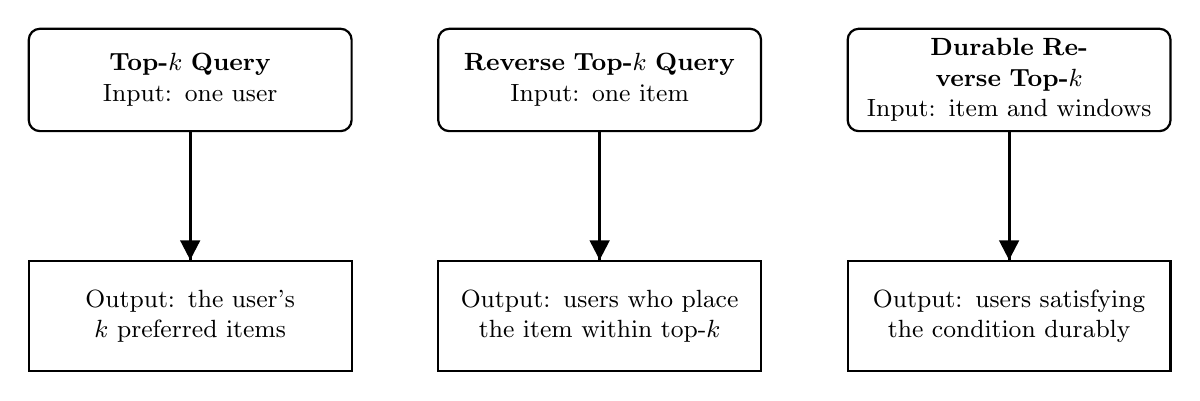
\begin{tikzpicture}[
font=\small,
querybox/.style={
rectangle,
rounded corners,
draw=black,
thick,
align=center,
minimum width=4.1cm,
minimum height=1.3cm,
text width=3.7cm
},
resultbox/.style={
rectangle,
draw=black,
thick,
align=center,
minimum width=4.1cm,
minimum height=1.4cm,
text width=3.7cm
}
]

\node[querybox] (topk) at (0,3)
{\textbf{Top-$k$ Query}\\Input: one user};

\node[resultbox] (topkresult) at (0,0)
{Output: the user's\\$k$ preferred items};

\node[querybox] (reverse) at (5.2,3)
{\textbf{Reverse Top-$k$ Query}\\Input: one item};

\node[resultbox] (reverseresult) at (5.2,0)
{Output: users who place\\the item within top-$k$};

\node[querybox] (durable) at (10.4,3)
{\textbf{Durable Reverse Top-$k$}\\Input: item and windows};

\node[resultbox] (durableresult) at (10.4,0)
{Output: users satisfying\\the condition durably};

% Arrow shafts (plain lines, no arrow-tip library required)
\draw[line width=1.1pt] (topk.south) -- (topkresult.north);
\draw[line width=1.1pt] (reverse.south) -- (reverseresult.north);
\draw[line width=1.1pt] (durable.south) -- (durableresult.north);

% Hand-drawn downward arrowheads (filled triangles, tip at the destination boundary)
\fill (topkresult.north) -- ++(0.13,0.25) -- ++(-0.26,0) -- cycle;
\fill (reverseresult.north) -- ++(0.13,0.25) -- ++(-0.26,0) -- cycle;
\fill (durableresult.north) -- ++(0.13,0.25) -- ++(-0.26,0) -- cycle;

\end{tikzpicture}
\caption{Conceptual comparison of top-$k$, reverse top-$k$, and durable reverse top-$k$ query processing}
\label{fig:query_comparison}
\end{figure}

Let $\mathcal{T}'\subseteq\mathcal{T}$ denote the set of temporal windows considered by a query, where

\begin{equation}
L'=\left|\mathcal{T}'\right|.
\label{eq:selected_window_count}
\end{equation}

Given a durability threshold $\tau\in(0,1]$, the minimum number of temporal windows in which the query item must satisfy the top-$k$ condition is

\begin{equation}
r=\left\lceil\tau L'\right\rceil.
\label{eq:durability_requirement}
\end{equation}

The durability count of user $u$ for query item $q$ is defined as

\begin{equation}
D(u,q,\mathcal{T}')
=
\sum_{t\in\mathcal{T}'}
\mathbb{I}
\left[
\operatorname{rank}(u,q,t)\leq k
\right],
\label{eq:durability_count}
\end{equation}

where $\mathbb{I}[\cdot]$ denotes the indicator function.

The durable reverse top-$k$ result set is defined as

\begin{equation}
\begin{aligned}
\operatorname{DRTop}\text{-}k(q,k,\tau,\mathcal{T}')
=
\bigl\{
u\in\mathcal{U}
\;\bigm|\;&
D(u,q,\mathcal{T}') \\
&\geq \left\lceil\tau L'\right\rceil
\bigr\}.
\end{aligned}
\label{eq:durable_reverse_topk}
\end{equation}

%----------------------------------------------------------------------------------------

\subsection{Problem Statement}
\label{subsec:problem_statement}

A straightforward exact solution evaluates every user in every selected temporal window and compares the query-item score with the scores of all available items. The approximate computational cost of this exhaustive verification is

\begin{equation}
O\left(nL'md\right),
\label{eq:exhaustive_complexity}
\end{equation}

where $n$ is the number of users, $L'$ is the number of selected temporal windows, $m$ is the number of items, and $d$ is the latent dimensionality. This cost becomes substantial for large recommendation datasets.

The central problem addressed in this thesis is stated as follows:

\begin{quote}
\textit{How can durable reverse top-$k$ users be identified efficiently over time-varying latent preferences without exhaustively verifying every user against every item in every temporal window?}
\end{quote}

The major challenges associated with the problem are summarized below:

\begin{itemize}

\item \textbf{Large search space:}
Exact verification may require evaluating thousands or millions of users against a large item collection.

\item \textbf{Multiple temporal windows:}
The top-$k$ condition must be evaluated repeatedly instead of being checked only once.

\item \textbf{Sparse interaction data:}
Some users may have limited or no ratings in particular temporal windows, making temporal preference construction difficult.

\item \textbf{Candidate-set selection:}
A very small candidate set reduces runtime but may exclude true durable users. A very large candidate set provides greater recall but reduces the computational benefit of filtering.

\item \textbf{Score-convention consistency:}
Dot-product preference scores follow a larger-is-better convention. Therefore, exact verification must compare the query-item score with the $k$-th largest score rather than the $k$-th smallest score.

\item \textbf{Accuracy--efficiency balance:}
The framework must provide substantial pruning and runtime improvement while maintaining high recall and precision.

\end{itemize}

To address these challenges, HyDART-RQ first applies the Durable Quantile Rank (DQR) filter to identify promising candidate users. Exact SSA or PRA verification is subsequently applied only to the filtered candidate set. The framework also supports an adaptive candidate budget so that the candidate-set size can be increased when a small fixed budget is likely to miss durable users.

The high-level workflow of HyDART-RQ is shown in Figure~\ref{fig:hydart_overview}.

\begin{figure}[H]
\centering
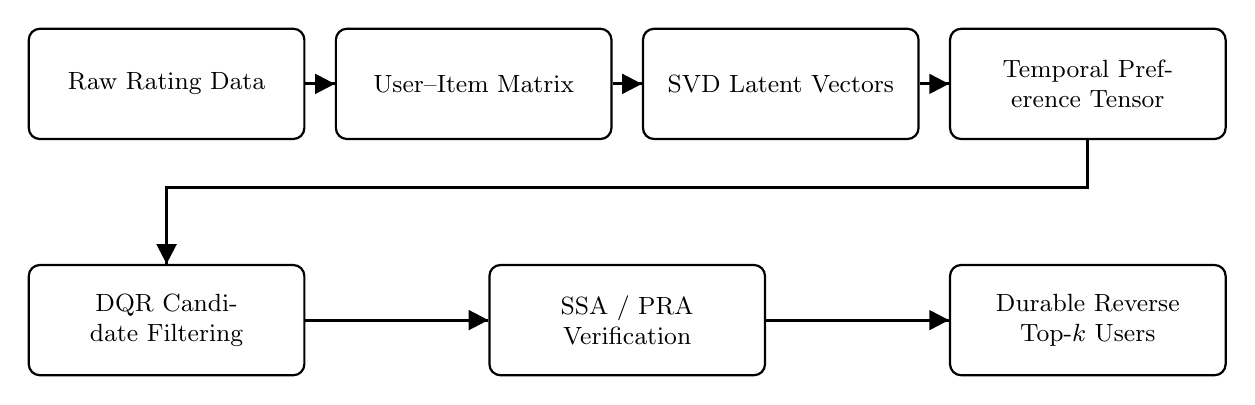
\begin{tikzpicture}[
font=\small,
stage/.style={
rectangle,
rounded corners,
draw=black,
thick,
align=center,
minimum width=3.5cm,
minimum height=1.4cm,
text width=3.2cm
}
]

\node[stage] (ratings) at (0,3)
{Raw Rating Data};

\node[stage] (matrix) at (3.9,3)
{User--Item Matrix};

\node[stage] (svd) at (7.8,3)
{SVD Latent Vectors};

\node[stage] (temporal) at (11.7,3)
{Temporal Preference Tensor};

\node[stage] (filter) at (0,0)
{DQR Candidate Filtering};

\node[stage] (verify) at (5.85,0)
{SSA / PRA Verification};

\node[stage] (result) at (11.7,0)
{Durable Reverse Top-$k$ Users};

% Arrow shafts (plain lines, no arrow-tip library required)
\draw[line width=1.1pt] (ratings.east) -- (matrix.west);
\draw[line width=1.1pt] (matrix.east) -- (svd.west);
\draw[line width=1.1pt] (svd.east) -- (temporal.west);
\draw[line width=1.1pt] (temporal.south) -- ++(0,-0.6) -| (filter.north);
\draw[line width=1.1pt] (filter.east) -- (verify.west);
\draw[line width=1.1pt] (verify.east) -- (result.west);

% Hand-drawn arrowheads (filled triangles, tip at the destination boundary)
\fill (matrix.west) -- ++(-0.25,0.13) -- ++(0,-0.26) -- cycle;
\fill (svd.west) -- ++(-0.25,0.13) -- ++(0,-0.26) -- cycle;
\fill (temporal.west) -- ++(-0.25,0.13) -- ++(0,-0.26) -- cycle;
\fill (filter.north) -- ++(0.13,0.25) -- ++(-0.26,0) -- cycle;
\fill (verify.west) -- ++(-0.25,0.13) -- ++(0,-0.26) -- cycle;
\fill (result.west) -- ++(-0.25,0.13) -- ++(0,-0.26) -- cycle;

\end{tikzpicture}
\caption{High-level workflow of the proposed HyDART-RQ framework}
\label{fig:hydart_overview}
\end{figure}

%----------------------------------------------------------------------------------------

\subsection{Motivating Example}
\label{subsec:motivating_example}

Consider a recommendation system containing five temporal windows. Let the query item be $q$, let $k=3$, and let the durability threshold be $\tau=0.6$. The minimum required number of successful windows is

\begin{equation}
\left\lceil\tau L\right\rceil
=
\left\lceil0.6\times5\right\rceil
=
3.
\label{eq:motivating_required_windows}
\end{equation}

Table~\ref{tab:motivating_example} presents the rank of query item $q$ for three users across five temporal windows.

\begin{table}[htbp]
\centering
\caption{Example of durable reverse top-$k$ qualification for $k=3$ and $\tau=0.6$}
\label{tab:motivating_example}
\small
\renewcommand{\arraystretch}{1.25}
\setlength{\tabcolsep}{5pt}
\begin{tabular}{|c|c|c|c|c|c|c|c|}
\hline
\textbf{User} &
\textbf{$t_1$} &
\textbf{$t_2$} &
\textbf{$t_3$} &
\textbf{$t_4$} &
\textbf{$t_5$} &
\textbf{Successful} &
\textbf{Durable} \\
\hline
$u_1$ & 2 & 3 & 5 & 2 & 3 & 4 & Yes \\
\hline
$u_2$ & 1 & 6 & 2 & 7 & 8 & 2 & No \\
\hline
$u_3$ & 4 & 2 & 3 & 5 & 1 & 3 & Yes \\
\hline
\end{tabular}
\end{table}

User $u_1$ ranks the query item within the top-$3$ in four windows and therefore satisfies the durability condition. User $u_2$ satisfies the top-$3$ condition in only two windows and is not durable. User $u_3$ satisfies the condition in exactly three windows and is therefore durable.

This example illustrates why a static reverse top-$k$ result can be misleading. If only the first temporal window were considered, user $u_2$ would appear highly relevant because the query item has rank $1$. However, the item does not remain highly ranked in the later windows. In contrast, user $u_3$ would be excluded in the first window even though the user satisfies the durability requirement over the complete interval.

For a large dataset, generating the complete rank sequence for every user requires extensive computation. HyDART-RQ therefore estimates which users are promising, eliminates unlikely users before exact verification, and retains a configurable number of candidates to preserve high result quality.

%----------------------------------------------------------------------------------------

\section{Objectives}
\label{sec:objectives}

The primary objective of this thesis is to develop an efficient hybrid framework for durable reverse top-$k$ query processing over time-varying preference data.

The specific objectives are as follows:

\begin{enumerate}

\item To formally define the durable reverse top-$k$ query problem using temporally varying latent user preferences.

\item To construct an end-to-end preprocessing pipeline that transforms timestamped rating data into sparse user--item matrices, latent item vectors, and temporal user-preference tensors.

\item To design and implement the Durable Quantile Rank (DQR) candidate filter for identifying users who are likely to satisfy the durability requirement.

\item To integrate the Sequential Search Algorithm (SSA) and the Pruning-based Algorithm (PRA) as exact durability verifiers within the HyDART-RQ framework.

\item To develop an adaptive candidate-budget mechanism that improves recall when a small fixed candidate set is insufficient.

\item To maintain consistency between the larger-is-better SVD scoring model and the ranking logic used by the filtering and verification components.

\item To evaluate the proposed framework using synthetic data and three real-world datasets: MovieLens, a subset of the Netflix Prize dataset, and Amazon Reviews 2023--Video Games.

\item To compare HyDART-RQ with full exact verification and alternative candidate-filtering strategies using recall, precision, exact-match ratio, pruning ratio, query-processing time, and speedup.

\item To investigate the sensitivity of the framework to parameters such as $k$, $\tau$, candidate factor $c$, latent dimension $d$, and number of temporal windows $L$.

\end{enumerate}

%----------------------------------------------------------------------------------------

\section{Scope}
\label{sec:scope}

The scope of this thesis is defined as follows:

\begin{itemize}

\item The research focuses on offline durable reverse top-$k$ queries over a predefined collection of query items.

\item User and item preferences are modeled using truncated SVD-based latent factors generated from sparse rating data.

\item Historical interactions are divided into equal-width temporal windows. The primary experiments use five windows, while sensitivity experiments examine alternative values.

\item The candidate-filtering methods include Durable Quantile Rank, Global Average, Union Window, and a legacy minimum-rank approach.

\item The DQR-based candidate filter forms the principal filtering component of HyDART-RQ.

\item SSA and PRA are used as exact durability verifiers for the selected candidate users.

\item Fixed and adaptive candidate-budget strategies are evaluated.

\item Experiments are conducted using synthetic data, MovieLens \texttt{ml\allowbreak-latest\allowbreak-small}, a selected Netflix Prize subset, and Amazon Reviews 2023--Video Games.

\item The framework is implemented in Python using NumPy, SciPy, pandas, and supporting scientific-computing libraries.

\item Evaluation is based on recall, precision, exact-match ratio, pruning ratio, average candidate count, query-processing time, and speedup.

\item Real-time streaming updates, distributed deployment, privacy-preserving recommendation, user-interface development, and causal analysis of user behaviour are outside the present scope.

\end{itemize}

Table~\ref{tab:scope_summary} summarizes the main boundaries of the study.

\begin{table}[htbp]
\centering
\caption{Summary of the research scope}
\label{tab:scope_summary}
\small
\renewcommand{\arraystretch}{1.25}
\setlength{\tabcolsep}{5pt}
\begin{tabularx}{\textwidth}{|p{3.3cm}|X|}
\hline
\textbf{Aspect} &
\textbf{Scope of the Thesis} \\
\hline
Query type &
Offline durable reverse top-$k$ query processing \\
\hline
Preference representation &
SVD-based latent user and item vectors \\
\hline
Temporal model &
Equal-width temporal windows and time-varying user vectors \\
\hline
Candidate filtering &
DQR, Global Average, Union Window, and legacy filtering \\
\hline
Exact verification &
Sequential Search Algorithm and Pruning-based Algorithm \\
\hline
Datasets &
Synthetic, MovieLens, Netflix Prize subset, and Amazon Video Games \\
\hline
Evaluation &
Recall, precision, pruning, exact matching, runtime, and speedup \\
\hline
Excluded areas &
Streaming updates, distributed execution, privacy-preserving processing, and user-interface design \\
\hline
\end{tabularx}
\end{table}

%----------------------------------------------------------------------------------------

\section{Unfamiliarity of the Problem, Topic, Solution}
\label{sec:unfamiliarity}

The proposed research is related to previous studies on reverse top-$k$ queries, approximate reverse ranking, temporal preference modeling, and durable query processing. However, HyDART-RQ is not a direct reproduction of any single existing approach. The originality of the work lies in the integration of durability-aware temporal rank filtering, exact candidate verification, adaptive candidate budgeting, and latent-factor recommendation within a unified processing framework.

The principal contributions are summarized in Table~\ref{tab:original_contributions}.

\begin{table}[htbp]
\centering
\caption{Original components and contributions of HyDART-RQ}
\label{tab:original_contributions}
\small
\renewcommand{\arraystretch}{1.25}
\setlength{\tabcolsep}{4pt}
\begin{tabularx}{\textwidth}{|p{3.5cm}|X|}
\hline
\textbf{Contribution} &
\textbf{Description} \\
\hline
Durable Quantile Rank filter &
Uses the temporal rank distribution of a query item to prioritize users who are more likely to satisfy the durability requirement. \\
\hline
Hybrid processing pipeline &
Combines approximate candidate filtering with exact SSA/PRA verification on a reduced user set. \\
\hline
Adaptive candidate budget &
Introduces a configurable minimum candidate count and boundary expansion to improve recall on sparse datasets. \\
\hline
Score-convention correction &
Ensures that all components consistently use the larger-is-better interpretation of SVD dot-product scores. \\
\hline
Unified data pipeline &
Processes synthetic, MovieLens, Netflix, and Amazon datasets through a common latent-factor and temporal-preference construction procedure. \\
\hline
Comprehensive evaluation &
Examines recall, precision, exact matching, pruning, runtime, speedup, scalability, and parameter sensitivity. \\
\hline
\end{tabularx}
\end{table}

The thesis does not claim that reverse top-$k$ queries, SVD, SSA, or PRA were independently invented in this work. These established concepts are acknowledged and adapted appropriately. The proposed contribution is the design and implementation of the complete HyDART-RQ framework and the investigation of how temporal candidate filtering and adaptive candidate selection can reduce the cost of exact durable reverse top-$k$ verification.

A particularly important contribution of the implementation is the identification and correction of a score-direction inconsistency. The original temporal verifiers used a smaller-is-better comparison, which is suitable for distance-based models. However, the SVD-based preference model used in this thesis produces dot-product similarity scores, for which larger values indicate stronger preferences. The verification condition was therefore corrected to compare the query-item score with the $k$-th largest item score. The corrected implementation was subsequently validated through correctness tests.

%----------------------------------------------------------------------------------------

\section{Project Planning}
\label{sec:project_planning}

The project was completed through a sequence of research, development, experimentation, validation, and documentation activities conducted over two academic semesters. Table~\ref{tab:project_plan} summarizes the major phases and their completion status.

\begin{table}[htbp]
\centering
\caption{Project planning and completion status}
\label{tab:project_plan}
\small
\renewcommand{\arraystretch}{1.25}
\setlength{\tabcolsep}{4pt}
\begin{tabularx}{\textwidth}{|p{1.0cm}|p{3.4cm}|X|p{2.0cm}|}
\hline
\textbf{Phase} &
\textbf{Activity} &
\textbf{Major Tasks} &
\textbf{Status} \\
\hline
1 &
Literature review &
Review of reverse top-$k$, approximate ranking, durable queries, and latent-factor recommendation &
Completed \\
\hline
2 &
Problem formulation &
Definition of temporal preferences, durability conditions, and evaluation requirements &
Completed \\
\hline
3 &
Data preparation &
Acquisition, cleaning, indexing, and temporal partitioning of datasets &
Completed \\
\hline
4 &
Baseline implementation &
Implementation and validation of full SSA, PRA, and static baselines &
Completed \\
\hline
5 &
Proposed framework &
Development of DQR filtering, hybrid processing, and adaptive candidate budgeting &
Completed \\
\hline
6 &
Experimentation &
Synthetic, MovieLens, Netflix, Amazon, robustness, and scalability experiments &
Completed \\
\hline
7 &
Testing and validation &
Correction of the score-direction inconsistency and execution of correctness tests &
Completed \\
\hline
8 &
Documentation &
Result analysis, figure preparation, and thesis writing &
Ongoing \\
\hline
\end{tabularx}
\end{table}

This thesis was completed as an individual capstone project. The author performed the literature review, problem formulation, data preparation, algorithm design, implementation, testing, experimentation, result analysis, visualization, and report preparation under the supervision of Dr.\ K.\ M.\ Azharul Hasan. The supervisor provided research guidance, technical suggestions, constructive feedback, and regular evaluation throughout the project.

%----------------------------------------------------------------------------------------

\section{Applications of the Work}
\label{sec:applications}

Durable reverse top-$k$ query processing has practical value in several application domains:

\begin{itemize}

\item \textbf{Targeted product promotion:}
E-commerce platforms can identify users who consistently rank a product or product category highly and direct promotional campaigns toward them.

\item \textbf{Audience discovery:}
Streaming platforms can identify users whose long-term preference profiles indicate sustained interest in a newly released movie, series, song, or game.

\item \textbf{Inventory planning:}
Retailers can estimate the durable audience of an item before adjusting stock levels or allocating promotional resources.

\item \textbf{Customer segmentation:}
Users can be separated into persistent-interest and temporary-interest groups according to the durability of their preferences.

\item \textbf{Gaming applications:}
Gaming platforms can identify players who consistently prefer related genres or franchises for beta testing, early access, or sequel promotion.

\item \textbf{Content and creator analysis:}
Social-media platforms can discover users who maintain sustained interest in particular creators, topics, or content categories.

\item \textbf{Long-term campaign evaluation:}
Marketing teams can distinguish short-term attention from durable user interest and prioritize audiences with more stable preferences.

\end{itemize}

Table~\ref{tab:application_summary} summarizes selected application scenarios.

\begin{table}[htbp]
\centering
\caption{Potential applications of durable reverse top-$k$ query processing}
\label{tab:application_summary}
\small
\renewcommand{\arraystretch}{1.25}
\setlength{\tabcolsep}{4pt}
\begin{tabularx}{\textwidth}{|p{3.2cm}|X|X|}
\hline
\textbf{Domain} &
\textbf{Query Item} &
\textbf{Possible Use} \\
\hline
E-commerce &
A product or product category &
Targeted promotion and inventory planning \\
\hline
Video streaming &
A movie, series, or genre &
Long-term audience discovery \\
\hline
Music streaming &
A song, artist, or music category &
Personalized campaign targeting \\
\hline
Gaming &
A game, franchise, or genre &
Beta-tester recruitment and sequel promotion \\
\hline
Social media &
A creator, topic, or content category &
Persistent audience identification \\
\hline
Market analysis &
A brand or product segment &
Distinguishing durable demand from temporary interest \\
\hline
\end{tabularx}
\end{table}

%----------------------------------------------------------------------------------------

\section{Organization of the Thesis}
\label{sec:thesis_organization}

This thesis is organized into seven chapters as follows:

\noindent
\textbf{Chapter I: Introduction.}
This chapter presents the research background, problem statement, motivating example, objectives, scope, originality, project planning, applications, and organization of the thesis.

\noindent
\textbf{Chapter II: Literature Review.}
This chapter reviews previous work related to reverse top-$k$ queries, approximate reverse ranking, durable query processing, temporal preferences, and matrix factorization. It also identifies the research gap addressed by HyDART-RQ.

\noindent
\textbf{Chapter III: Methodology.}
This chapter presents the complete HyDART-RQ methodology, including data preprocessing, latent-factor construction, temporal preference modeling, DQR filtering, SSA/PRA verification, and adaptive candidate budgeting.

\noindent
\textbf{Chapter IV: Implementation, Results and Discussions.}
This chapter describes the implementation environment, datasets, experimental settings, evaluation metrics, quantitative results, qualitative examples, and analysis of the proposed framework.

\noindent
\textbf{Chapter V: Societal, Health, Environment, Safety, Ethical, Legal and Cultural Issues.}
This chapter discusses intellectual-property considerations, dataset ethics, privacy, software licensing, sustainability, and the wider societal implications of the research.

\noindent
\textbf{Chapter VI: Addressing Complex Engineering Problems and Activities.}
This chapter explains the complex engineering problems associated with the project and the technical activities undertaken to design, implement, test, and validate the framework.

\noindent
\textbf{Chapter VII: Conclusions.}
This chapter summarizes the major findings and contributions, discusses the limitations of the current framework, and presents recommendations and future research directions.
